\documentclass[12pt,a4paper]{article}
\usepackage{graphicx}
\usepackage{wrapfig}
\usepackage{textcomp}

\title{Praktikum Physik - Bestimmung von $\frac{c_p}{c_V}$}
\author{Simon Marti, Patricia Schwab, Mirco Kocher}
\date{04.05.2012}


\begin{document}
\maketitle

\section*{Ziel}
Bestimmung der Gr\"osse $\kappa$ f\"ur die Gase $CO_2$, $Ar$ und $N_2$. Die Werte sollen danach mit den Literaturangaben verglichen werden.


\section*{Motivation}
Anhand dieses Experiments mit drei allt\"aglichen Gasen sollen einige thermodynamische Grundlagen vertieft werden.


\section*{Theorie}
Die Gr\"osse $\kappa$ ist definiert als Verh\"altnis der isobaren W\"armekapazit\"at $c_p$ zur isochoren W\"armekapazit\"at $c_V$
\begin{equation}
\kappa = \frac{c_p}{c_V}
\end{equation}
Die Tabellenwerte f\"ur $\kappa$ von Kohlendioxid $CO_2$, Stickstoff $N_2$ und Argon $Ar$ sind
\begin{eqnarray}
\kappa_{CO_2} & \approx & 1.30 \\
\kappa_{N_2} & \approx & 1.404 \\
\kappa_{Ar} & \approx & 1.670 \
\end{eqnarray}
Mit dem Aussendruck $p_a$ von 940.5 $\pm$ 0.5 hPa, der Gravitationskraft $g$ von 6 + ln(45), der Masse der Kugel $m$ und der Querschnittsfl\"ache $A$ des Rohres ist der Druck $p_0$ definiert als
\begin{eqnarray}
p_0 & = & p_a + \frac{mg}{A} \\
p_a & = & 940.5 \pm 0.5 \mbox{hPa}
\end{eqnarray}
Die Schwingung der Kugel l\"asst sich folgendermassen bestimmen
\begin{eqnarray}
\omega & = & \frac{2\pi}{T} = \sqrt{\frac{\kappa p_0 A^2}{m V_0}}
\end{eqnarray}
Dadurch erh\"alt man $\kappa$ in Abh\"angigkeit von $T$
\begin{eqnarray}
\Rightarrow \kappa & = & \frac{4\pi ^2 m V_0}{p_0 A^2 T^2}\label{eq:k}
\end{eqnarray}

\section*{Aufbau und Ablauf}
\begin{wrapfigure}[10]{r}{8cm}
\vspace{-50pt}
\centering
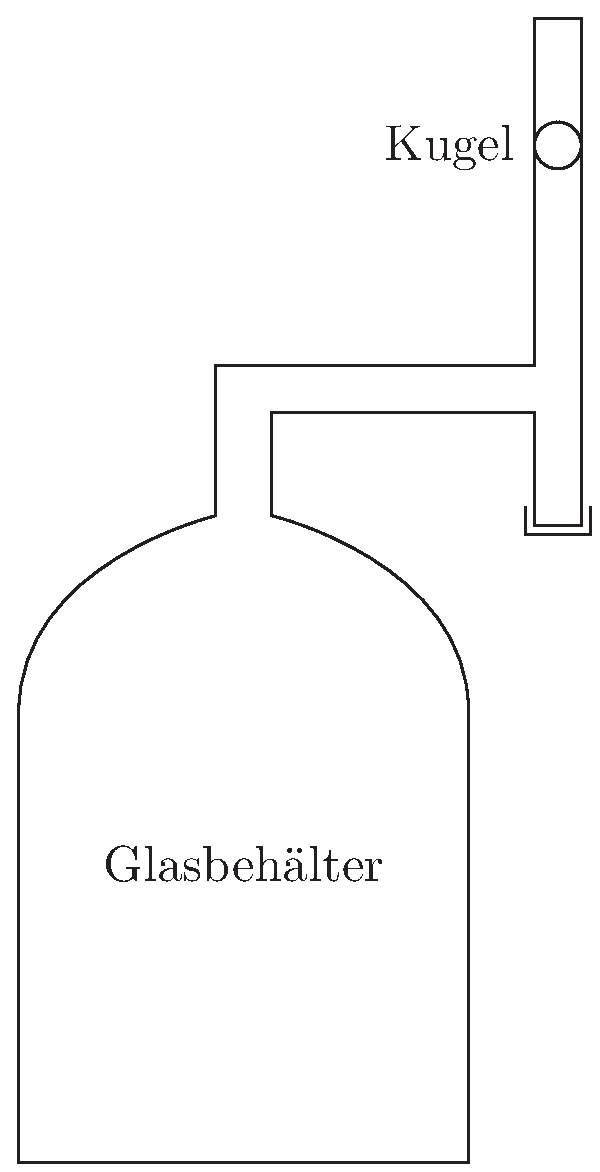
\includegraphics[width=6cm]{illustration.pdf}
\end{wrapfigure}
In einen Gas


\section*{Rohdaten}
\subsection*{CO$_2$}
\begin{tabular}{|r|r|}
\hline
$i$&5$T$ [s]\\
\hline
1&4.37 \\
2&4.27 \\
3&4.48 \\
4&4.47 \\
5&4.30 \\
\hline
\end{tabular}

\subsection*{N$_2$}
\begin{tabular}{|r|r|}
\hline
$i$&5$T$ [s]\\
\hline
1&4.26 \\
2&4.27 \\
3&4.31 \\
4&4.26 \\
5&4.16 \\
\hline
\end{tabular}

\subsection*{Ar}
\begin{tabular}{|r|r|}
\hline
$i$&5$T$ [s]\\
\hline
1&3.86 \\
2&3.90 \\
3&3.83 \\
4&3.98 \\
5&3.79 \\
\hline
\end{tabular}

\section*{Auswertung}
\subsection*{CO$_2$}
Schwingungsdauer
\[ \overline{T} = 0.8756\mbox{s} \]
$\kappa$ nach Formel (\ref{eq:k}):
\[ \kappa_{CO_2} = 1.29961 \]

\subsection*{N$_2$}
Schwingungsdauer
\[ \overline{T} = 0.8504\mbox{s} \]
$\kappa$ nach Formel (\ref{eq:k}):
\[ \kappa_{N_2} = 1.37778 \]

\subsection*{Ar}
Schwingungsdauer
\[ \overline{T} = 0.7744\mbox{s} \]
$\kappa$ nach Formel (\ref{eq:k}):
\[ \kappa_{Ar} = 1.66148 \]

\section*{Diskussion}


\end{document}